\section{Datensatz}
\label{sec:Datensatz}

Da kein passender Datensatz gefunden wurde, musste dieser auch als Teil des Projekts erstellt werden.
Das Ziel war es für viele verschiedene Orte innerhalb europäischer Grenzen ein Satellitenbild und eine passende Maske zu sammeln.
Die Maske soll dabei die Pixel markieren, die zu größeren Wasserflächen wie Seen, Teichen, Flüssen, Kanälen oder Küstenabschnitten gehören.
Zusätzlich werden zu jedem Ort einige Metadaten wie die Koordinaten und das zugehörige Land in einer CSV Datei gespeichert.
Ein Beispiel vom erzeugten Datensatz ist in \autoref{fig:datensatz_beispiel} zu sehen.

\begin{figure}
    \centering
    \begin{subfigure}{0.3\textwidth}
        \centering
        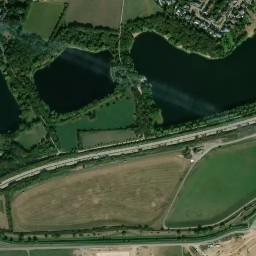
\includegraphics[width=\textwidth]{images/datensatz_beispiel_satellit.jpg}
        \caption{Satellitenbild}
        \label{fig:datensatz_beispiel_satellit}
    \end{subfigure}
    \begin{subfigure}{0.3\textwidth}
        \centering
        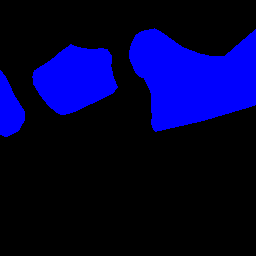
\includegraphics[width=\textwidth]{images/datensatz_beispiel_maske.png}
        \caption{Maskenbild}
        \label{fig:datensatz_beispiel_maske.png}
    \end{subfigure}
    \caption{\\Beispiel des Datensatzes an den Koordinaten %
            ${x_\text{Tile} = 16998}$, ${y_\text{Tile} = 10927}$, ${z_\text{Tile} = 15}$, %
            ${x_\text{Geo} = 6,751°}$, ${y_\text{Geo} = 51,293°}$. %
            (in Deutschland) \copyright Mapbox, \copyright OpenStreetMap}
    \label{fig:datensatz_beispiel}
\end{figure}

Die Datensatz-Erstellung wurde mit Python automatisiert und wird im Folgenden erläutert.

Die Daten wurden nicht in einer Sitzung, sondern immer in kleinen Paketen gesammelt.
Dafür wurden zuerst gleichverteilte Zufallszahlen für Längengrad $x_\text{Geo}$ und Breitengrad $y_\text{Geo}$ (also in geographischen Koordinaten) 
im Bereich ${x_\text{Geo} \in [-10,49° \,,\, 40,27°]}$, ${y_\text{Geo} \in [34,51° \,,\, 71,20°]}$ gezogen.
Dieser Bereich ist eine grobe Begrenzung für Europa.
Für jeden so gezogenen Ort wurde mithilfe der groben Ländergrenzen\footnote{\url{https://www.naturalearthdata.com/downloads/110m-cultural-vectors/110m-admin-0-countries/}} des \enquote{Natural Earth} Projektes überprüft, 
ob dieser Ort innerhalb eines europäischen Landes liegt. \cite{natural_earth}
Hierbei wurden Russland und Island nicht miteinbezogen.

Ziel war es viele Satellitenbilder zu sammeln, die Wasser enthalten.
Da in Europa allerdings das Verhältnis von Wasser- zu Landfläche sehr gering ist, musste vor dem Herunterladen der Wassergehalt des Bildes überprüft werden.
Dies wurde mithilfe der Daten der \enquote{Mapbox Vector Tiles API}\footnote{\url{https://docs.mapbox.com/api/maps/}\label{mapbox_api}} überprüft. \cite{mapbox}
Ein Ort wurde nur dann akzeptiert, wenn dieser nicht schon zuvor gezogen wurde und das Bild sowohl einen Wasseranteil als auch einen Landanteil hat.

Für jeden akzeptierten Ort wurde dann mithilfe der \enquote{Mapbox Raster Tiles API}\footref{mapbox_api} ein Satellitenbild heruntergeladen.
Außerdem wurde von diesem Ort mithilfe der \enquote{Mapbox Static Tiles API}\footref{mapbox_api} und einem selbst angepassten Kartenstil ein Maskenbild für den Wassergehalt heruntergeladen.\cite{mapbox}
Mapbox verwendet die Kartendaten von \enquote{OpenStreetMap} und somit stammen auch die Daten der Maskenbilder daher.\cite{OpenStreetMap}

An dieser Stelle scheint es sinnvoll zu erwähnen, dass die Maskenbilder teilweise Fehler enthalten und Gewässer nur sehr grob oder auch falsch zugeordnet sind. 

In der Bereitstellung von digitalen Karten und geographischen Daten wird heutzutage vermehrt das Konzept sogenannter \enquote{Tiles} verwendet.\cite{tiles}
Hier ist eine Zoom-Stufe $z_\text{Tile}$ anzugeben und die Welt wird in $4^{z_\text{Tile}}$ gleichgroße Quadrate(\enquote{Tiles}) aufgeteilt.
Jedem dieser Quadrate wird eine $x_\text{Tile}$- und eine $y_\text{Tile}$-Koordinate zugeordnet.

Während der Erstellung des Datensatzes musste zwischen einigen Koordinatensystemen gewechselt werden, aber die Koordinaten der \enquote{Tiles} waren ausschlaggebend für die heruntergeladenen Bilder.
Jedes Bild im Datensatz wurde mit einer Zoom-Stufe $z_\text{Tile} = 15$ generiert und entspricht genau einem \enquote{Tile}.

Der Datensatz enthielt am Ende des Projektes 57931 Satellitenbilder und dazu passende Maskenbilder.
Jedes Bild hatte eine Auflösung von 256 x 256 Pixel.
